\documentclass[11pt]{article}
\usepackage[margin=1in]{geometry}
\usepackage{amsmath,amssymb}
\usepackage{algorithm}
\usepackage{algpseudocode}
\usepackage{fancyhdr}
\usepackage{enumerate}
\usepackage{graphicx}
\usepackage[colorlinks=true,linkcolor=blue,urlcolor=blue]{hyperref}

\newcommand{\hwnum}{10}

% page header, same as the posted solutions
\pagestyle{fancy}
\fancyhf{}
\lhead{EECS 376: Foundations of Computer Science\\University of Michigan, Fall 2026}
\rhead{\vspace{\baselineskip}Solutions to Homework \hwnum}
\cfoot{\thepage}
\setlength{\headheight}{28pt}

% pseudocode labels
\renewcommand{\algorithmicrequire}{\textbf{Input:}}
\renewcommand{\algorithmicensure}{\textbf{Output:}}

% notation
\newcommand{\set}[1]{\left\{#1\right\}}
\newcommand{\abs}[1]{\left|#1\right|}
\newcommand{\lp}{\leq_p}
\newcommand{\cproblem}[1]{\textsc{#1}}
\renewcommand{\P}{\textsf{P}}
\newcommand{\NP}{\textsf{NP}}
\newcommand{\SAT}{\cproblem{SAT}}
\newcommand{\SSUM}{\cproblem{Subset-Sum}}
\newcommand{\KNAPSACK}{\cproblem{Knapsack}}
\newcommand{\MaxCut}{\textsf{MAX-CUT}}
\newcommand{\OPT}{\mathrm{OPT}}
\newcommand{\ALG}{\mathrm{ALG}}
\newcommand{\Ex}{\mathrm{E}}
\newcommand{\algo}[1]{\textsc{#1}}

% one part per page for Gradescope
\newcommand{\qpage}[1]{\clearpage\noindent\textbf{\large #1}\par\medskip}

\begin{document}

\noindent\textbf{\large Q0 Before you start; before you submit}\par\medskip

I did not collaborate with anyone on this homework.

\qpage{Q1 Self assessment}

I chose HW9 Question 4(b), explaining why the Cook-Levin statement proves that $\SAT$ is $\NP$-hard.
My overall argument is right, but the justification of one step is muddled.
Here is what I submitted:

\begin{center}
  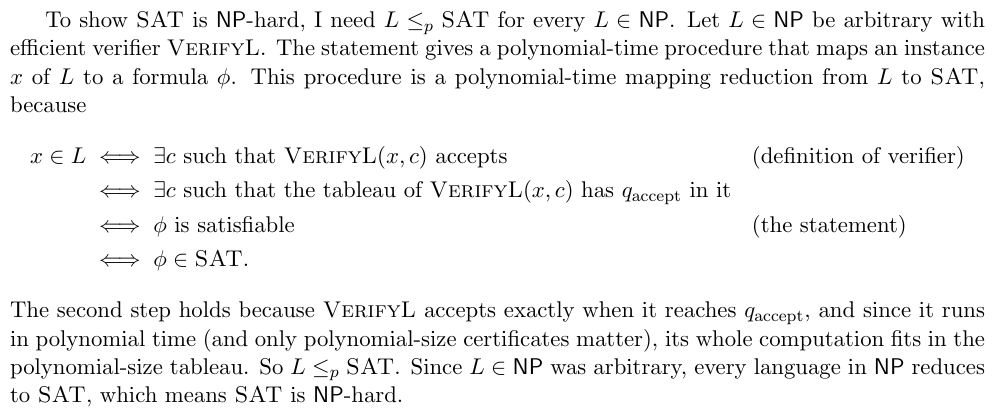
\includegraphics[width=0.8\linewidth]{hw9_q4b.png}
\end{center}

\textbf{What was deficient.}
The second equivalence in my chain (``$\textsc{VerifyL}(x, c)$ accepts $\iff$ the tableau of $\textsc{VerifyL}(x, c)$ has $q_{\text{accept}}$ in it'') is exactly what the tableau is built to show, and the posted solution just says it in one phrase: $\textsc{VerifyL}$ accepts, ``meaning that its tableau contains $q_{\text{accept}}$.''
Instead, I wrote a sentence that mixes in two things that are not needed here and are not explained: the claim that ``only polynomial-size certificates matter,'' and the claim that the computation fits in the tableau.
These are facts about how $\phi$ is \emph{constructed}, which the problem already gives us inside the quoted statement, so bringing them up in my answer only makes the reader wonder whether I am proving something extra.
The parenthetical ``only polynomial-size certificates matter'' is also stated without any reason, so it reads like a gap even though nothing depends on it.
Finally, the conclusion ``So $L \lp \SAT$'' does not say clearly that the two properties of a mapping reduction (polynomial time, and $x \in L \iff \phi \in \SAT$) both hold.

\textbf{How to fix it.}
I would drop the extra sentence and justify the second step simply by the definition of the tableau: the tableau of $\textsc{VerifyL}(x, c)$ records its computation, so it contains $q_{\text{accept}}$ exactly when $\textsc{VerifyL}(x, c)$ accepts.
Then I would end with one sentence that checks both conditions: the map $x \mapsto \phi$ is computable in polynomial time (given by the statement) and $x \in L \iff \phi \in \SAT$ (the chain), so $L \lp \SAT$.
Since $L \in \NP$ was arbitrary, $\SAT$ is $\NP$-hard.

\qpage{Q2.1 Indicator variables and linearity of expectation (a)}

Let $V$ be the vertex set, $\abs{V} = n$.
For each unordered pair $\set{u, v}$ of distinct vertices, let
\[
  X_{uv} = \begin{cases} 1 & \text{if } (u, v) \text{ is an edge of } G_{n,p}, \\ 0 & \text{otherwise.} \end{cases}
\]
Then $\Ex[X_{uv}] = \Pr[(u, v) \text{ is an edge}] = p$.
The number of edges is $X = \sum_{\set{u, v}} X_{uv}$, summed over all $\binom{n}{2}$ pairs.
By linearity of expectation,
\[
  \Ex[X] = \sum_{\set{u, v}} \Ex[X_{uv}] = \binom{n}{2} p = \frac{n(n-1)}{2}\, p.
\]

\qpage{Q2.2 Indicator variables and linearity of expectation (b)}

Fix a vertex $v$.
Its degree is the number of edges at $v$, so with the same indicators as in part (a),
\[
  \deg(v) = \sum_{u \in V,\ u \neq v} X_{uv}.
\]
There are $n - 1$ vertices $u \neq v$, and $\Ex[X_{uv}] = p$ for each.
By linearity of expectation,
\[
  \Ex[\deg(v)] = \sum_{u \neq v} \Ex[X_{uv}] = (n - 1)\, p.
\]

\qpage{Q2.3 Indicator variables and linearity of expectation (c)}

For each set $T = \set{u, v, w}$ of three distinct vertices, let
\[
  Y_T = \begin{cases} 1 & \text{if } T \text{ is a triangle in } G_{n,p}, \\ 0 & \text{otherwise.} \end{cases}
\]
$T$ is a triangle exactly when all three edges $(u, v)$, $(v, w)$, $(u, w)$ are present.
These are three different pairs, so the three edges are included independently, each with probability $p$.
So
\[
  \Ex[Y_T] = \Pr[T \text{ is a triangle}] = p \cdot p \cdot p = p^3.
\]
The number of triangles is $Y = \sum_T Y_T$, summed over all $\binom{n}{3}$ sets of three vertices.
By linearity of expectation,
\[
  \Ex[Y] = \sum_T \Ex[Y_T] = \binom{n}{3} p^3 = \frac{n(n-1)(n-2)}{6}\, p^3.
\]

\qpage{Q2.4 Indicator variables and linearity of expectation (d)}

Let $Y$ be the number of triangles, as in part (c).
$Y$ is a nonnegative random variable, and $n^3 p^2 > 0$ since $n > 0$ and $p > 0$.
So Markov's inequality applies:
\[
  \Pr[Y \geq n^3 p^2] \leq \frac{\Ex[Y]}{n^3 p^2}
  = \frac{n(n-1)(n-2)\, p^3}{6\, n^3 p^2}
  = \frac{(n-1)(n-2)}{n^2} \cdot \frac{p}{6}.
\]
If $n \geq 2$, then $0 \leq n - 1 < n$ and $0 \leq n - 2 < n$, so $\frac{(n-1)(n-2)}{n^2} \leq 1$.
If $n = 1$, then $(n-1)(n-2) = 0$.
In both cases $\frac{(n-1)(n-2)}{n^2} \leq 1$, so
\[
  \Pr[Y \geq n^3 p^2] \leq \frac{p}{6}.
\]

\qpage{Q3.1 You're Too Tall!! (a)}

Number the positions $1, \ldots, n$ from left to right.
For each position $i$, let $D_i = 1$ if the tree at position $i$ dies, and $D_i = 0$ otherwise.
The number of dead trees is $D = \sum_{i=1}^n D_i$.

I use the following fact: since the order is uniformly random and the heights are distinct, for any fixed set of $k$ positions, every one of the $k!$ relative orders of the heights at those positions is equally likely.
(For each relative order, swapping the trees within those positions gives a bijection between the orderings that produce it and the orderings that produce any other relative order, so they all have the same number of orderings.)
In particular, each of the $k$ positions is equally likely to hold the shortest of those $k$ trees, with probability $1/k$.

\textbf{End trees ($i = 1$ or $i = n$).}
An end tree dies if it is shorter than its only neighbor.
Looking at the $2$ positions (the end and its neighbor), the end tree is the shorter one with probability $1/2$.
So $\Ex[D_1] = \Ex[D_n] = 1/2$.

\textbf{Middle trees ($2 \leq i \leq n-1$).}
The tree at $i$ dies if it is shorter than both neighbors, i.e., it is the shortest among the $3$ positions $i-1, i, i+1$.
This has probability $1/3$, so $\Ex[D_i] = 1/3$.

By linearity of expectation,
\[
  \Ex[D] = \Ex[D_1] + \Ex[D_n] + \sum_{i=2}^{n-1} \Ex[D_i] = \frac{1}{2} + \frac{1}{2} + \frac{n-2}{3} = \frac{n+1}{3}.
\]
(Check: for $n = 2$, exactly one tree, the shorter one, dies, and $\frac{2+1}{3} = 1$.)

\qpage{Q3.2 You're Too Tall!! (b)}

Number the positions in the line $1, \ldots, n$ from front to back.
Every complaint comes from a pair of students: a student at position $j$ complains once about each taller student at a position $i < j$.
So the total number of complaints is the number of pairs of positions $i < j$ such that the student at position $i$ is taller than the student at position $j$.

For each pair of positions $i < j$, let
\[
  X_{ij} = \begin{cases} 1 & \text{if the student at } i \text{ is taller than the student at } j, \\ 0 & \text{otherwise.} \end{cases}
\]
The total number of complaints is $X = \sum_{i < j} X_{ij}$.

Since the line is uniformly random and heights are distinct, the two relative orders of the students at positions $i$ and $j$ are equally likely (swapping the two students at $i$ and $j$ is a bijection between the lineups with each order).
So $\Ex[X_{ij}] = \Pr[\text{student at } i \text{ is taller}] = 1/2$.

There are $\binom{n}{2}$ pairs $i < j$, so by linearity of expectation,
\[
  \Ex[X] = \sum_{i < j} \Ex[X_{ij}] = \binom{n}{2} \cdot \frac{1}{2} = \frac{n(n-1)}{4}.
\]
(Check with the example from the problem: $n = 3$ gives $\frac{3 \cdot 2}{4} = 1.5$, halfway between the fewest possible complaints, $0$, and the most, $3$, which is what we expect by symmetry.)

\qpage{Q4.1 Fair coin-flip challenge (a)}

In one iteration, $b_1$ and $b_2$ come from two independent calls to $\algo{GetBiasedBit}$.
The algorithm returns $0$ exactly when $b_1 = 0$ and $b_2 = 1$, and returns $1$ exactly when $b_1 = 1$ and $b_2 = 0$.
By independence,
\begin{align*}
  \Pr[\text{returns } 0] &= \Pr[b_1 = 0] \cdot \Pr[b_2 = 1] = (1 - p)\, p, \\
  \Pr[\text{returns } 1] &= \Pr[b_1 = 1] \cdot \Pr[b_2 = 0] = p\, (1 - p).
\end{align*}
These are equal.

So in each iteration the algorithm is equally likely to return $0$ or $1$ (and otherwise it goes to the next iteration, which uses new independent bits), which is why the final output is unbiased.

\qpage{Q4.2 Fair coin-flip challenge (b)}

Let $A$ be the event that the first attempt succeeds, so $\Pr[A] = q$ and $\Pr[\overline{A}] = 1 - q$.
By the law of total expectation,
\[
  \Ex[X] = \Pr[A] \cdot \Ex[X \mid A] + \Pr[\overline{A}] \cdot \Ex[X \mid \overline{A}].
\]

\textbf{If the first attempt succeeds}, the experiment stops after $1$ attempt, so $\Ex[X \mid A] = 1$.

\textbf{If the first attempt fails}, we have used $1$ attempt and we start over.
The remaining attempts are independent of the first one and each succeeds with probability $q$, so the number of remaining attempts $X'$ has the same distribution as $X$.
So $X = 1 + X'$ and $\Ex[X \mid \overline{A}] = 1 + \Ex[X'] = 1 + \Ex[X]$.

Putting this together,
\[
  \Ex[X] = q \cdot 1 + (1 - q)(1 + \Ex[X]).
\]

\textbf{Solving.}
First, $\Ex[X]$ is finite: $X \geq k$ only if the first $k - 1$ attempts all fail, so $\Pr[X \geq k] = (1-q)^{k-1}$ and
$\Ex[X] = \sum_{k \geq 1} \Pr[X \geq k] = \sum_{k \geq 1} (1-q)^{k-1}$, a geometric series with ratio $1 - q < 1$, which converges.
So we can rearrange the equation:
\[
  \Ex[X] = q + (1 - q) + (1 - q)\Ex[X] = 1 + (1 - q)\Ex[X]
  \quad\Longrightarrow\quad q\, \Ex[X] = 1
  \quad\Longrightarrow\quad \Ex[X] = \frac{1}{q}.
\]

\qpage{Q4.3 Fair coin-flip challenge (c)}

Each iteration of the \textbf{while} loop is an attempt that succeeds (returns) when $(b_1, b_2) = (0, 1)$ or $(1, 0)$.
By part (a), this happens with probability
\[
  q = (1-p)p + p(1-p) = 2p(1-p),
\]
and $q > 0$ because $0 < p < 1$.
Different iterations use different calls to $\algo{GetBiasedBit}$, so they succeed independently.
So the number of iterations $X$ is geometric with success probability $q$, and by part (b),
\[
  \Ex[X] = \frac{1}{2p(1-p)}.
\]
Each iteration makes exactly $2$ calls to $\algo{GetBiasedBit}$, so the number of calls is $2X$, and by linearity of expectation
\[
  \Ex[\text{number of calls}] = 2\,\Ex[X] = \frac{2}{2p(1-p)} = \frac{1}{p(1-p)}.
\]

\qpage{Q5.1 Randomized \MaxCut\ (a)}

For each edge $e = (u, v) \in E$, let $X_e = 1$ if $e$ crosses the cut ($e \in C(S)$), and $X_e = 0$ otherwise.
Then $\abs{C(S)} = \sum_{e \in E} X_e$.

There are no self-loops, so $u \neq v$, and $u, v$ are put into $S$ independently with probability $1/2$ each.
The edge crosses the cut exactly when one endpoint is in $S$ and the other is not:
\[
  \Ex[X_e] = \Pr[u \in S, v \notin S] + \Pr[u \notin S, v \in S] = \frac{1}{2} \cdot \frac{1}{2} + \frac{1}{2} \cdot \frac{1}{2} = \frac{1}{2}.
\]
By linearity of expectation,
\[
  \Ex[\abs{C(S)}] = \sum_{e \in E} \Ex[X_e] = \frac{\abs{E}}{2}.
\]
Every cut, in particular a maximum cut, has at most $\abs{E}$ crossing edges, so $\OPT \leq \abs{E}$.
Therefore
\[
  \Ex[\abs{C(S)}] = \frac{\abs{E}}{2} \geq \frac{\OPT}{2},
\]
so the algorithm is a $1/2$-approximation in expectation.

\qpage{Q5.2 Randomized \MaxCut\ (b)}

Let $\varepsilon > 0$.
If $\abs{E} = 0$, then $(1-\varepsilon)\abs{E}/2 = 0 \leq \abs{C(S)}$ always, so the probability is $1 \geq \frac{\varepsilon}{1+\varepsilon}$.
So assume $\abs{E} \geq 1$.

Markov's inequality bounds the probability that a nonnegative variable is \emph{large}, but here we want $\abs{C(S)}$ to be large with good probability.
So I apply Markov to the number of edges that do \emph{not} cross the cut,
\[
  Y = \abs{E} - \abs{C(S)}.
\]
$Y \geq 0$ since $C(S) \subseteq E$, and by part (a), $\Ex[Y] = \abs{E} - \abs{E}/2 = \abs{E}/2$.

The cut is too small exactly when $Y$ is large:
\[
  \abs{C(S)} < (1-\varepsilon)\frac{\abs{E}}{2}
  \iff Y > \abs{E} - (1-\varepsilon)\frac{\abs{E}}{2} = (1+\varepsilon)\frac{\abs{E}}{2}.
\]
Since $(1+\varepsilon)\abs{E}/2 > 0$, Markov's inequality gives
\[
  \Pr\left[\abs{C(S)} < (1-\varepsilon)\frac{\abs{E}}{2}\right]
  \leq \Pr\left[Y \geq (1+\varepsilon)\frac{\abs{E}}{2}\right]
  \leq \frac{\Ex[Y]}{(1+\varepsilon)\abs{E}/2}
  = \frac{\abs{E}/2}{(1+\varepsilon)\abs{E}/2}
  = \frac{1}{1+\varepsilon}.
\]
Taking the complement,
\[
  \Pr\left[\abs{C(S)} \geq (1-\varepsilon)\frac{\abs{E}}{2}\right] \geq 1 - \frac{1}{1+\varepsilon} = \frac{\varepsilon}{1+\varepsilon}.
\]

\qpage{Q5.3 Randomized \MaxCut\ (c)}

If $\abs{E} = 0$, every cut has size $0 \geq \abs{E}/2$, so exactly $1$ attempt is needed.
So assume $\abs{E} \geq 1$.

Let $q = \Pr[\abs{C(S)} \geq \abs{E}/2]$ be the probability that one run succeeds.

\textbf{Lower bound on $q$.}
Take any $\varepsilon$ with $0 < \varepsilon < 1/\abs{E}$.
Then $\varepsilon\abs{E} < 1$, which is the same as $(1-\varepsilon)\abs{E}/2 > (\abs{E}-1)/2$.
If $\abs{C(S)} \geq (1-\varepsilon)\abs{E}/2$, then $\abs{C(S)} > (\abs{E}-1)/2$, i.e., $2\abs{C(S)} > \abs{E} - 1$.
Both sides are integers, so $2\abs{C(S)} \geq \abs{E}$, i.e., $\abs{C(S)} \geq \abs{E}/2$.
So by part (b),
\[
  q \geq \Pr\left[\abs{C(S)} \geq (1-\varepsilon)\frac{\abs{E}}{2}\right] \geq \frac{\varepsilon}{1+\varepsilon}.
\]
This holds for every $\varepsilon \in (0, 1/\abs{E})$, and $\frac{\varepsilon}{1+\varepsilon}$ increases with $\varepsilon$, so letting $\varepsilon$ approach $1/\abs{E}$,
\[
  q \geq \frac{1/\abs{E}}{1 + 1/\abs{E}} = \frac{1}{\abs{E} + 1}.
\]
(For example, the single choice $\varepsilon = \frac{1}{\abs{E}+1}$ already gives $q \geq \frac{1}{\abs{E}+2}$.)

\textbf{Expected number of attempts.}
Each run of the algorithm uses new independent random choices, so the runs succeed independently, each with probability $q > 0$.
So the number of attempts is geometric with success probability $q$, and by Q4(b),
\[
  \Ex[\text{number of attempts}] = \frac{1}{q} \leq \abs{E} + 1.
\]

\qpage{Q6.1 More Knapsack! (a)}

I show that $\SSUM \lp \KNAPSACK$. Since $\SSUM$ is $\NP$-hard, this shows that $\KNAPSACK$ is also $\NP$-hard.

\textbf{Step 1: the reduction.}
The idea is to make each number an item whose weight and value are both equal to the number, and to set both the capacity and the budget to $s$.
Then ``weight at most $s$'' and ``value at least $s$'' together mean ``sum exactly $s$.''

\begin{algorithmic}[1]
  \Require{A multiset $A = \set{a_1, \ldots, a_n}$ of integers $\geq 0$, and an integer $s$}
  \Ensure{An instance of $\KNAPSACK$}
  \Function{$f$}{$A, s$}
    \If{$s < 0$} \Return a fixed ``no'' instance, e.g.\ $(W = (), V = (), C = 0, K = 1)$
    \EndIf
    \State Remove every $a_i$ with $a_i > s$; let $a_1, \ldots, a_{n'}$ be the remaining numbers
    \For{$i = 1, \ldots, n'$}
      \State $W_i \gets a_i$, \quad $V_i \gets a_i$
    \EndFor
    \State \Return $(W, V, C = s, K = s)$
  \EndFunction
\end{algorithmic}

The fixed instance has no items, so the only choice is $S = \emptyset$ with value $0 < 1$; it is a ``no'' instance.
If $s < 0$, $(A, s) \notin \SSUM$ too, since every subset of $A$ has a nonnegative sum.
The values are nonnegative integers, and after removing the large numbers every $W_i \leq C$, so the output is a valid $\KNAPSACK$ instance.
Removing the numbers $a_i > s$ does not change the answer: all numbers are $\geq 0$, so a subset containing some $a_i > s$ has sum $> s$, and no subset that sums to $s$ uses it.
So from now on assume $s \geq 0$ and every $a_i \leq s$.

\textbf{Step 2: polynomial time.}
The reduction makes one pass over $A$ to remove large numbers and copy each remaining number twice, and copies $s$ twice.
This takes time linear in the size of $(A, s)$.

\textbf{Step 3a: $(A, s) \in \SSUM \Longrightarrow f(A, s) \in \KNAPSACK$.}
Let $I$ be a submultiset of $A$ with $\sum_{a \in I} a = s$, and let $S$ be the set of indices of the items in $I$ (as noted, $I$ uses only numbers $\leq s$, which were kept).
Then
\[
  \sum_{i \in S} W_i = \sum_{a \in I} a = s \leq C
  \qquad\text{and}\qquad
  \sum_{i \in S} V_i = \sum_{a \in I} a = s \geq K.
\]
So $f(A, s) \in \KNAPSACK$.

\textbf{Step 3b: $f(A, s) \in \KNAPSACK \Longrightarrow (A, s) \in \SSUM$.}
Let $S \subseteq \set{1, \ldots, n'}$ satisfy $\sum_{i \in S} W_i \leq C$ and $\sum_{i \in S} V_i \geq K$.
Since $W_i = V_i = a_i$ and $C = K = s$, this says
\[
  s \leq \sum_{i \in S} a_i \leq s,
  \qquad\text{so}\qquad \sum_{i \in S} a_i = s.
\]
The numbers $a_i$ for $i \in S$ form a submultiset of $A$ with sum $s$, so $(A, s) \in \SSUM$.

By Steps 2, 3a, and 3b, $\SSUM \lp \KNAPSACK$, so $\KNAPSACK$ is $\NP$-hard.

\qpage{Q6.2 More Knapsack! (b)}

No, it does not prove $\P = \NP$.

An algorithm is polynomial time if its running time is polynomial in the \emph{size of the input}, i.e., the number of bits needed to write it down.
The capacity $C$ is written in binary, so it takes only about $\log_2 C$ bits.
The running time $O(nC)$ is polynomial in the \emph{value} of $C$, but $C = 2^{\log_2 C}$ is exponential in the number of bits of $C$.

For example, take $n$ items and capacity $C = 2^n$ (with weights and values of at most $n$ bits each).
The input has size polynomial in $n$, about $O(n^2)$ bits, but the algorithm takes time about $n \cdot 2^n$, which is exponential in the input size.
So the DP algorithm is only \emph{pseudo-polynomial}, it does not show $\KNAPSACK \in \P$, and we cannot conclude that $\P = \NP$.

\qpage{Q7.1 Zingerman's catering (a)}

\textbf{Optimal allocation.}
Give order $7$ (time $3$) to chef A, orders $1, 2, 3$ to chef B, and orders $4, 5, 6$ to chef C.
Each chef works $3$, so the completion time is $3$.
This is optimal: any allocation has completion time at least $t_7 = 3$, because the chef who gets order $7$ works at least $3$ (this is also part (b)).
So $\OPT = 3$.

\textbf{Sequence 1: allocate order $7$ first.}
All chefs are at $0$, so order $7$ goes to some chef, say A; the loads are $(3, 0, 0)$.
Then the six orders of time $1$ are allocated.
As long as B or C has load less than $3$, the earliest finisher is B or C (A is at $3$), so the loads go (up to swapping B and C)
\[ (3,1,0),\ (3,1,1),\ (3,2,1),\ (3,2,2),\ (3,3,2),\ (3,3,3). \]
The completion time is $3$, and the approximation ratio is $3/3 = 1$.

\textbf{Sequence 2: allocate order $7$ last.}
The six orders of time $1$ are allocated first.
Each goes to a chef with the smallest load, so the loads go (up to renaming chefs)
\[ (1,0,0),\ (1,1,0),\ (1,1,1),\ (2,1,1),\ (2,2,1),\ (2,2,2). \]
Now all chefs are at $2$, so order $7$ goes to one of them, giving loads $(5, 2, 2)$.
The completion time is $5$, and the approximation ratio is $5/3$.

So depending on the order in which orders are allocated, \algo{GreedyAllocate} gets completion time $3$ (ratio $1$) or $5$ (ratio $5/3$).

\qpage{Q7.2 Zingerman's catering (b)}

Consider an optimal allocation, and let $t_j = \max\set{t_1, \ldots, t_m}$.
Order $j$ is allocated to some chef.
That chef's total time includes $t_j$, and all times are nonnegative, so that chef's total is at least $t_j$.
The completion time is the maximum total over all chefs, so it is at least that chef's total.
So
\[
  \OPT \geq t_j = \max\set{t_1, \ldots, t_m}.
\]

\qpage{Q7.3 Zingerman's catering (c)}

Assume $m \leq n$.

\textbf{Each order goes to a chef whose current load is $0$.}
When the algorithm allocates its $k$th order ($k \leq m \leq n$), only $k - 1 < n$ orders have been allocated, so at most $k - 1$ chefs have any orders, and some chef has load $0$.
Loads are nonnegative, so the earliest finisher has load $0$, and the order goes to a chef with load $0$.

\textbf{Every chef's final load is a single order time.}
Take any chef $c$ that gets at least one order, and let $j$ be the last order $c$ gets.
When $j$ was allocated, $c$ had load $0$ by the claim above, and $c$ gets nothing after $j$.
So the final load of $c$ is $0 + t_j = t_j \leq \max_i t_i$.
Chefs with no orders have load $0$.

So $\ALG \leq \max\set{t_1, \ldots, t_m} \leq \OPT$ by part (b).
Also $\ALG \geq \OPT$ since $\OPT$ is the minimum over all allocations.
Hence $\ALG = \OPT$, and \algo{GreedyAllocate} returns an optimal allocation.

\qpage{Q7.4 Zingerman's catering (d)}

Consider an optimal allocation, and let $L_1, \ldots, L_n$ be the total times of the chefs.
Every order is allocated to exactly one chef, so
\[
  \sum_{c=1}^{n} L_c = \sum_{j=1}^{m} t_j.
\]
The maximum of $n$ numbers is at least their average, so
\[
  \OPT = \max_c L_c \geq \frac{1}{n} \sum_{c=1}^{n} L_c = \frac{1}{n} \sum_{j=1}^{m} t_j.
\]

\qpage{Q7.5 Zingerman's catering (e)}

Let $c$ be a chef who finishes last, so $c$'s final load is $\ALG$.
If $c$ has no orders, then $\ALG = 0 \leq 2 \cdot \OPT$.
Otherwise, let $j$ be the last order allocated to $c$.

\textbf{Load of $c$ before order $j$.}
$c$ gets no orders after $j$, so just before $j$ was allocated, $c$'s load was $\ALG - t_j$.

\textbf{Bounding $\ALG - t_j$.}
The algorithm gave $j$ to $c$ because $c$ would finish earliest, i.e., $c$ had the smallest load at that moment.
So at that moment every chef had load at least $\ALG - t_j$, and the total load of all chefs was at least $n(\ALG - t_j)$.
The orders allocated at that moment do not include $j$, so their total time is at most $\sum_{i \neq j} t_i \leq \sum_{i=1}^m t_i$.
Hence
\[
  n(\ALG - t_j) \leq \sum_{i=1}^m t_i
  \quad\Longrightarrow\quad
  \ALG - t_j \leq \frac{1}{n} \sum_{i=1}^m t_i \leq \OPT
\]
by part (d).

\textbf{Bounding $t_j$.}
By part (b), $t_j \leq \max_i t_i \leq \OPT$.

\textbf{Conclusion.}
\[
  \ALG = (\ALG - t_j) + t_j \leq \OPT + \OPT = 2 \cdot \OPT.
\]

\qpage{Q8 (Optional extra credit) Disk storage}

\textbf{Algorithm.}
\begin{algorithmic}[1]
  \Require{File sizes $\ell_1, \ldots, \ell_n \geq 0$ and capacity $C$}
  \Function{TwoDisks}{$\ell_1, \ldots, \ell_n, C$}
    \State Sort the files by size so that $\ell_1 \leq \ell_2 \leq \cdots \leq \ell_n$ (renaming indices)
    \State Let $k$ be the largest number with $\ell_1 + \cdots + \ell_k \leq 2C$ \Comment{$k = 0$ if $\ell_1 > 2C$}
    \State Let $r$ be the largest number with $r \leq k$ and $\ell_1 + \cdots + \ell_r \leq C$
    \State $S_1 \gets \set{1, \ldots, r}$
    \State $S_2 \gets \set{r + 2, \ldots, k}$ \Comment{skip file $r + 1$; empty if $r \geq k - 1$}
    \State \Return $(S_1, S_2)$
  \EndFunction
\end{algorithmic}

\textbf{Runtime.}
Sorting takes $O(n \log n)$ time, and $k$ and $r$ can be found with one pass over the prefix sums, so the algorithm runs in polynomial time.

Write $P_t = \ell_1 + \cdots + \ell_t$ for the sum of the $t$ smallest files ($P_0 = 0$).
Since sizes are nonnegative, $P_t$ is nondecreasing in $t$.

\textbf{The output is a valid solution.}
$S_1$ and $S_2$ are disjoint.
$S_1$ has total size $P_r \leq C$ by the choice of $r$.
If $r \geq k - 1$, $S_2$ is empty.
Otherwise $r + 1 \leq k$, and by the maximality of $r$, $P_{r+1} > C$.
So $S_2$ has total size
\[
  \ell_{r+2} + \cdots + \ell_k = P_k - P_{r+1} < 2C - C = C,
\]
using $P_k \leq 2C$.
So both disks are within capacity.

\textbf{$\ALG \geq k - 1$.}
If $r = k$, the algorithm stores $k$ files.
Otherwise it stores all of $1, \ldots, k$ except file $r + 1$, which is $k - 1$ files.

\textbf{$\OPT \leq k$.}
Take any solution $(S_1^*, S_2^*)$ and let $t = \abs{S_1^* \cup S_2^*}$.
The stored files have total size at most $C + C = 2C$.
Any $t$ files have total size at least that of the $t$ smallest files, $P_t$.
So $P_t \leq 2C$, and by the maximality of $k$ (and since $P$ is nondecreasing), $t \leq k$.
So $\OPT \leq k$.

\textbf{Conclusion.}
$\ALG \geq k - 1 \geq \OPT - 1$.

\end{document}
